\documentclass[letterpaper,12pt]{article}

\usepackage[margin=1.25in]{geometry}
\usepackage{amsmath, amssymb}
\usepackage{graphicx}
\usepackage{ulem}
\usepackage{enumitem}
\usepackage{listings}

\lstset{language=R}

\begin{document}

\begin{flushleft}
    \textbf{Homework 2} \\
    \textbf{Course }: S520 Intro to Statistics \\
    \textbf{Author }: Jack McShane \\
    \textbf{Date }: February 8, 2022 \\
\end{flushleft}

\begin{flushleft}
\textbf{Question 1}: Suppose 5 cards are dealt from a standard deck of playing cards. How many hands are possible?
\end{flushleft}
\begin{center}
    In this instance, the order in which the cards are dealt does not matter. We are therefore looking for the number of combinations, not the number of permutations.
\end{center}
\begin{align*}
    C(n,r) &= \frac{P(n,r)}{P(r,r)}\\
    &=\frac{P(52,5)}{P(5,5)}\\
    &=\frac{52*51*50*49*48}{5!} \\
    &=\uuline{2598960}
\end{align*} \\


\begin{flushleft}
\textbf{Question 2}: Suppose that X is a random variable with cdf:
\end{flushleft}
\begin{align*}
    F(y) = 
    \begin{cases}
        0 & y \leq 0 \\
        \frac{y}{3} & y \in [0, 1) \\
        \frac{2}{3} & y \in [1, 2] \\
        \frac{y}{3} & y \in [2, 3] \\
        1 & y \geq 3
    \end{cases}
\end{align*}

\begin{center}
    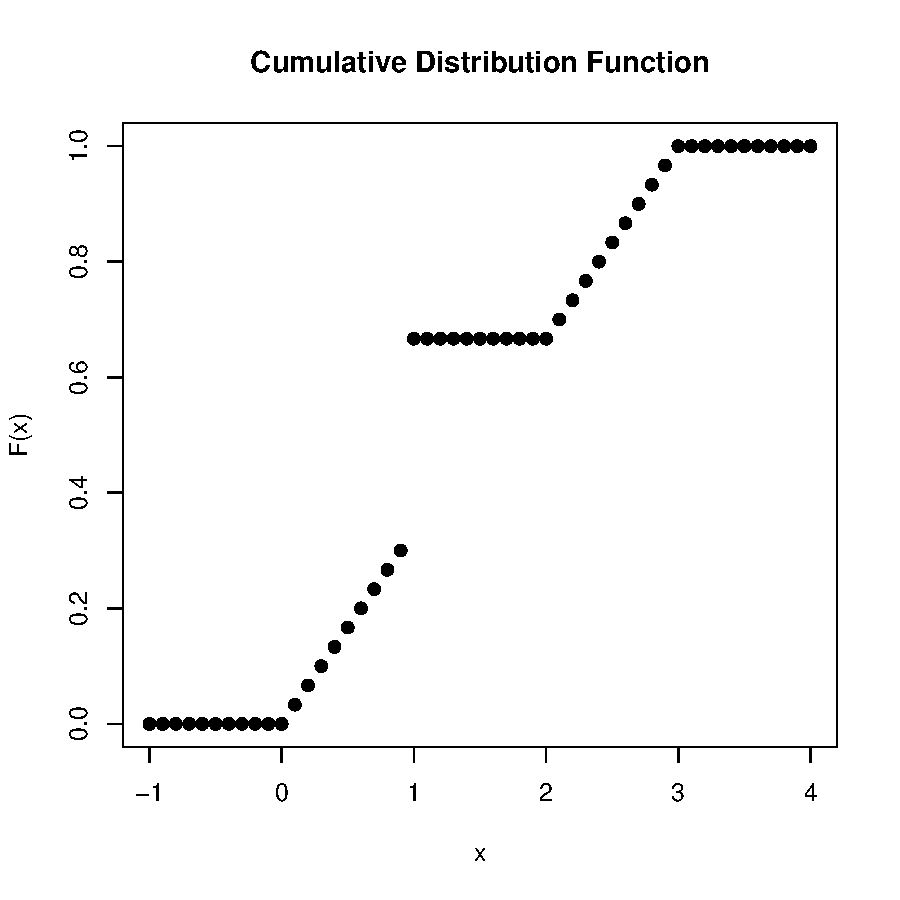
\includegraphics{piecewise.pdf}
\end{center}


\begin{enumerate}[label=(\alph*)]
    \item{What is P(X $>$ .5) ?} \\
        \begin{align*}
            P(X > .5) & = 1 - P(X \leq .5) \\
            & = 1 - F(.5) \\
            & = 1 - \frac{.5}{3} \\
            & = 1 - \frac{1}{6} \\
            & = \uuline{\frac{5}{6}} \\
        \end{align*}
    \item{What is P(2 $<$ X $\leq$ 3) ?} \\
        \begin{align*}
            P(2 < X \leq 3) & = P(X \leq 3) - P(X \leq 2) \\
            & = F(3) - F(2) \\
            & = 1 - \frac{2}{3} \\
            & = \uuline{\frac{1}{3}} \\
        \end{align*}
    \item{What is P(.5 $<$ X $\leq$ 2.5) ?} \\
        \begin{align*}
            P(.5 < X \leq 2.5) & = P(X \leq 2.5) - P(X \leq .5) \\
            & = F(2.5) - F(.5) \\
            & = \frac{5}{6} - \frac{1}{6} \\
            & = \uuline{\frac{2}{3}} \\
        \end{align*}
    \item{What is P(X = 1) ?} \\
        \begin{align*}
            P(X = 1) & = P(X \leq 1) - P(X < 1) \\
            & = F(1) - F(1^{-}) \\
            & = \frac{2}{3} - \frac{1}{3} \\
            & = \uuline{\frac{1}{3}} \\
        \end{align*}
\end{enumerate}


\begin{flushleft}
    \textbf{Question 3}: Suppose that X(S) = {1, 3, 4, 6} and P(X = 1) = P(X = 6) = .1, \\
    P(X = 3) = P(X = 4) = .4.
\end{flushleft}
\begin{enumerate}[label=(\alph*)]
    \item{Determine the pmf.} \\
        \begin{align*}
            pmf(X) = 
            \begin{cases}
                .1 & X = 1 \\
                .4 & X = 3 \\
                .4 & X = 4 \\
                .1 & X = 6 \\
                0 & otherwise
            \end{cases}
        \end{align*}
        \begin{center}
            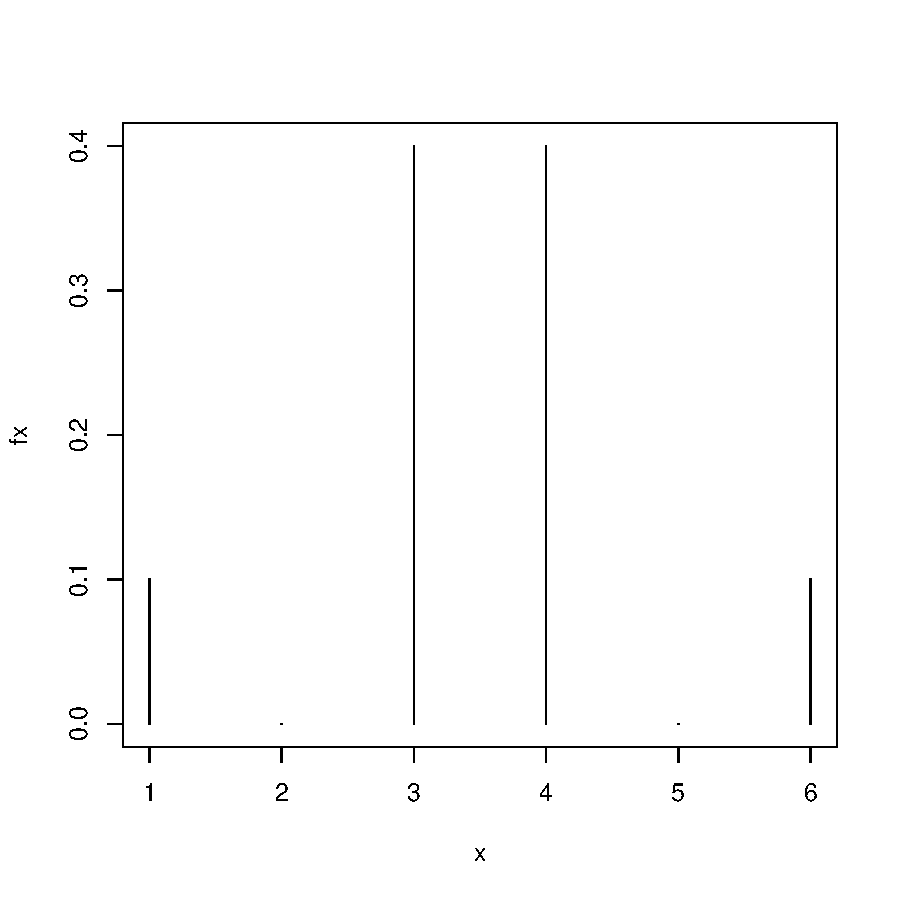
\includegraphics{pmf.pdf}
        \end{center}
    \item{Determine the cdf.} \\
        \begin{align*}
            F(X=x) = 
            \begin{cases}
                0 & x < 1 \\
                .1 & x \in [1, 3) \\
                .5 & x \in [3, 4) \\
                .9 & x \in [4, 6) \\
                1 & x \geq 6
            \end{cases}
        \end{align*}
        \begin{center}
            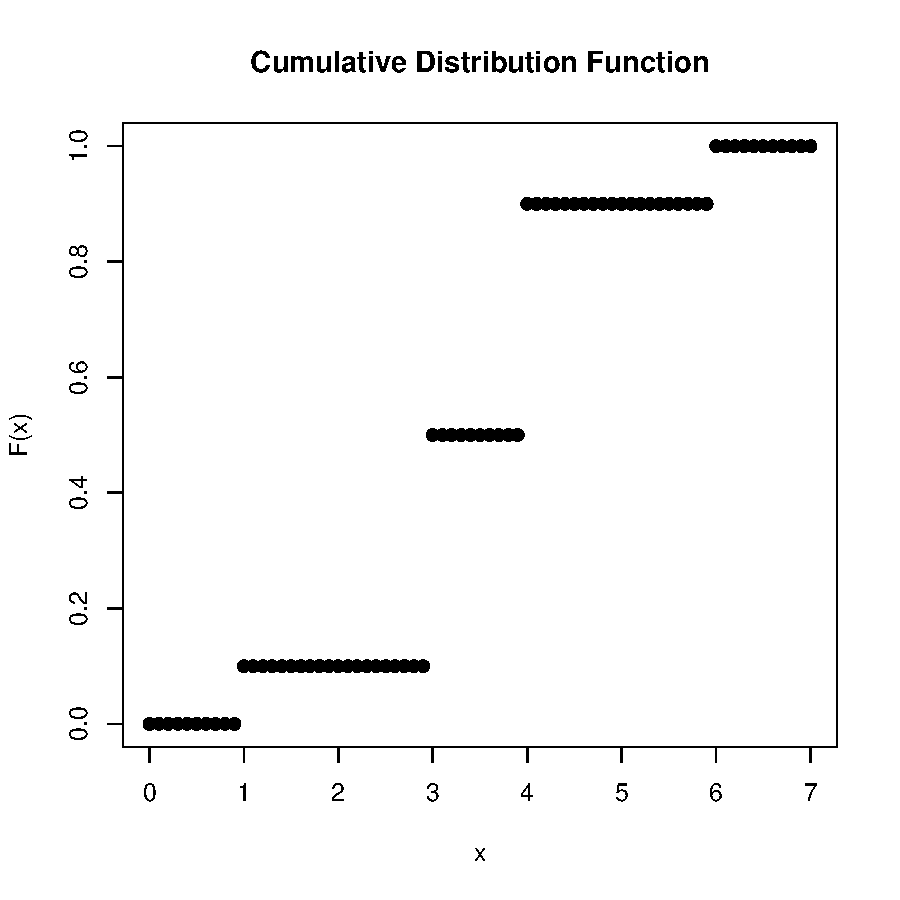
\includegraphics{cdf.pdf}
        \end{center}
\end{enumerate}

\begin{flushleft}
    \textbf{Question 4}: In a multiple choice exam, there are 20 questions and each question \\
    has three choices. If someone is totally unprepared and randomly chooses answers. \\
    Let Y be the number of questions (s)he guesses correctly.
\end{flushleft}
\begin{enumerate}[label=(\alph*)]
    \item{What is the distribution of Y?}
        \begin{center}
            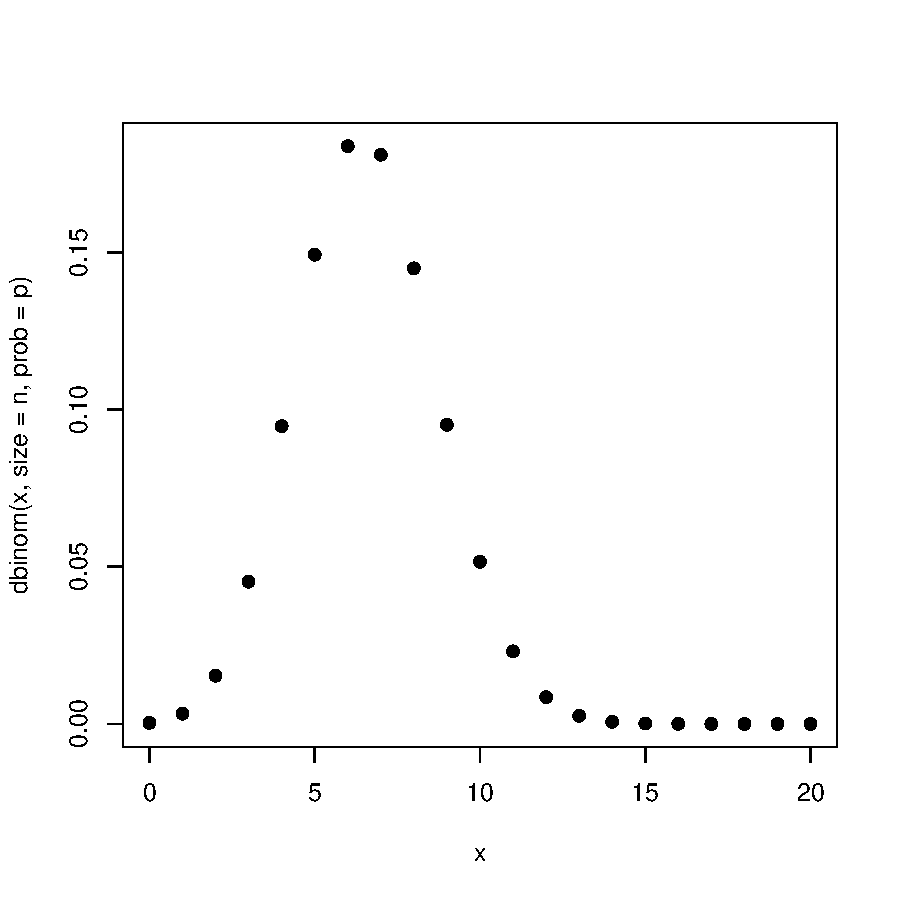
\includegraphics{dist.pdf}
            \begin{lstlisting}
                x <- 0:20
                n <- 20
                p <- .33
                plot(x, dbinom(x, size=n, prob=p), pch=19)
            \end{lstlisting}
        \end{center}
    \item{What is P(Y=6)?}
        \begin{align*}
            P(Y=6) = \uuline{.184}
        \end{align*}
        \begin{center}
            \begin{lstlisting}
                dbinom(6, size=n, prob=p)
            \end{lstlisting}
        \end{center}
    \item{What is P(Y $\leq$ 6)?}
        \begin{align*}
            P(Y \leq 6) = \uuline{.492}
        \end{align*}
        \begin{center}
            \begin{lstlisting}
                sum(dbinom(0:6, size=n, prob=p))
            \end{lstlisting}
        \end{center}
    \item{What is P(Y $>$ 6)?}
        \begin{align*}
            P(Y > 6) & = 1 - P(Y \leq 6) \\
            & = \uuline{.508}
        \end{align*}
        \begin{center}
            \begin{lstlisting}
                1 - dbinom(0:6, size=20, prob=p)
            \end{lstlisting}
        \end{center}
\end{enumerate}


\end{document}
